\documentclass[10pt,a4paper,onecolumn]{article}
\usepackage{marginnote}
\usepackage{graphicx}
\usepackage{xcolor}
\usepackage{authblk,etoolbox}
\usepackage{titlesec}
\usepackage{calc}
\usepackage{tikz}
\usepackage{hyperref}
\hypersetup{colorlinks,breaklinks,
            urlcolor=[rgb]{0.0, 0.5, 1.0},
            linkcolor=[rgb]{0.0, 0.5, 1.0}}
\usepackage{caption}
\usepackage{tcolorbox}
\usepackage{amssymb,amsmath}
\usepackage{ifxetex,ifluatex}
\usepackage{seqsplit}
\usepackage{fixltx2e} % provides \textsubscript
\usepackage[
  backend=biber,
%  style=alphabetic,
%  citestyle=numeric
]{biblatex}
\bibliography{paper.bib}



% --- Page layout -------------------------------------------------------------
\usepackage[top=3.5cm, bottom=3cm, right=1.5cm, left=1.0cm,
            headheight=2.2cm, reversemp, includemp, marginparwidth=4.5cm]{geometry}

% --- Default font ------------------------------------------------------------
% \renewcommand\familydefault{\sfdefault}

% --- Style -------------------------------------------------------------------
\renewcommand{\bibfont}{\small \sffamily}
\renewcommand{\captionfont}{\small\sffamily}
\renewcommand{\captionlabelfont}{\bfseries}

% --- Section/SubSection/SubSubSection ----------------------------------------
\titleformat{\section}
  {\normalfont\sffamily\Large\bfseries}
  {}{0pt}{}
\titleformat{\subsection}
  {\normalfont\sffamily\large\bfseries}
  {}{0pt}{}
\titleformat{\subsubsection}
  {\normalfont\sffamily\bfseries}
  {}{0pt}{}
\titleformat*{\paragraph}
  {\sffamily\normalsize}


% --- Header / Footer ---------------------------------------------------------
\usepackage{fancyhdr}
\pagestyle{fancy}
\fancyhf{}
%\renewcommand{\headrulewidth}{0.50pt}
\renewcommand{\headrulewidth}{0pt}
\fancyhead[L]{\hspace{-0.75cm}\includegraphics[width=5.5cm]{C:/Users/npjun/AppData/Local/R/win-library/4.4/rticles/rmarkdown/templates/joss/resources/JOSS-logo.png}}
\fancyhead[C]{}
\fancyhead[R]{}
\renewcommand{\footrulewidth}{0.25pt}

\fancyfoot[L]{\footnotesize{\sffamily Piñeiro-Juncal et.
al., (2025). BlueCarbon R package: Estimation of Organic Carbon Stocks
and Sequestration Rates From Soil Core
Data. \textit{Journal of Open Source Software}, (), . \href{https://doi.org/}{https://doi.org/}}}


\fancyfoot[R]{\sffamily \thepage}
\makeatletter
\let\ps@plain\ps@fancy
\fancyheadoffset[L]{4.5cm}
\fancyfootoffset[L]{4.5cm}

% --- Macros ---------

\definecolor{linky}{rgb}{0.0, 0.5, 1.0}

\newtcolorbox{repobox}
   {colback=red, colframe=red!75!black,
     boxrule=0.5pt, arc=2pt, left=6pt, right=6pt, top=3pt, bottom=3pt}

\newcommand{\ExternalLink}{%
   \tikz[x=1.2ex, y=1.2ex, baseline=-0.05ex]{%
       \begin{scope}[x=1ex, y=1ex]
           \clip (-0.1,-0.1)
               --++ (-0, 1.2)
               --++ (0.6, 0)
               --++ (0, -0.6)
               --++ (0.6, 0)
               --++ (0, -1);
           \path[draw,
               line width = 0.5,
               rounded corners=0.5]
               (0,0) rectangle (1,1);
       \end{scope}
       \path[draw, line width = 0.5] (0.5, 0.5)
           -- (1, 1);
       \path[draw, line width = 0.5] (0.6, 1)
           -- (1, 1) -- (1, 0.6);
       }
   }

% --- Title / Authors ---------------------------------------------------------
% patch \maketitle so that it doesn't center
\patchcmd{\@maketitle}{center}{flushleft}{}{}
\patchcmd{\@maketitle}{center}{flushleft}{}{}
% patch \maketitle so that the font size for the title is normal
\patchcmd{\@maketitle}{\LARGE}{\LARGE\sffamily}{}{}
% patch the patch by authblk so that the author block is flush left
\def\maketitle{{%
  \renewenvironment{tabular}[2][]
    {\begin{flushleft}}
    {\end{flushleft}}
  \AB@maketitle}}
\makeatletter
\renewcommand\AB@affilsepx{ \protect\Affilfont}
%\renewcommand\AB@affilnote[1]{{\bfseries #1}\hspace{2pt}}
\renewcommand\AB@affilnote[1]{{\bfseries #1}\hspace{3pt}}
\makeatother
\renewcommand\Authfont{\sffamily\bfseries}
\renewcommand\Affilfont{\sffamily\small\mdseries}
\setlength{\affilsep}{1em}


\ifnum 0\ifxetex 1\fi\ifluatex 1\fi=0 % if pdftex
  \usepackage[T1]{fontenc}
  \usepackage[utf8]{inputenc}

\else % if luatex or xelatex
  \ifxetex
    \usepackage{mathspec}
  \else
    \usepackage{fontspec}
  \fi
  \defaultfontfeatures{Ligatures=TeX,Scale=MatchLowercase}

\fi
% use upquote if available, for straight quotes in verbatim environments
\IfFileExists{upquote.sty}{\usepackage{upquote}}{}
% use microtype if available
\IfFileExists{microtype.sty}{%
\usepackage{microtype}
\UseMicrotypeSet[protrusion]{basicmath} % disable protrusion for tt fonts
}{}

\usepackage{hyperref}
\hypersetup{unicode=true,
            pdftitle={BlueCarbon R package: Estimation of Organic Carbon Stocks and Sequestration Rates From Soil Core Data},
            pdfborder={0 0 0},
            breaklinks=true}
\urlstyle{same}  % don't use monospace font for urls
\usepackage{graphicx,grffile}
\makeatletter
\def\maxwidth{\ifdim\Gin@nat@width>\linewidth\linewidth\else\Gin@nat@width\fi}
\def\maxheight{\ifdim\Gin@nat@height>\textheight\textheight\else\Gin@nat@height\fi}
\makeatother
% Scale images if necessary, so that they will not overflow the page
% margins by default, and it is still possible to overwrite the defaults
% using explicit options in \includegraphics[width, height, ...]{}
\setkeys{Gin}{width=\maxwidth,height=\maxheight,keepaspectratio}
\IfFileExists{parskip.sty}{%
\usepackage{parskip}
}{% else
\setlength{\parindent}{0pt}
\setlength{\parskip}{6pt plus 2pt minus 1pt}
}
\setlength{\emergencystretch}{3em}  % prevent overfull lines
\setcounter{secnumdepth}{0}
% Redefines (sub)paragraphs to behave more like sections
\ifx\paragraph\undefined\else
\let\oldparagraph\paragraph
\renewcommand{\paragraph}[1]{\oldparagraph{#1}\mbox{}}
\fi
\ifx\subparagraph\undefined\else
\let\oldsubparagraph\subparagraph
\renewcommand{\subparagraph}[1]{\oldsubparagraph{#1}\mbox{}}
\fi


% tightlist command for lists without linebreak
\providecommand{\tightlist}{%
  \setlength{\itemsep}{0pt}\setlength{\parskip}{0pt}}


% Pandoc citation processing
%From Pandoc 3.1.8
% definitions for citeproc citations
\NewDocumentCommand\citeproctext{}{}
\NewDocumentCommand\citeproc{mm}{%
  \begingroup\def\citeproctext{#2}\cite{#1}\endgroup}
\makeatletter
 % allow citations to break across lines
 \let\@cite@ofmt\@firstofone
 % avoid brackets around text for \cite:
 \def\@biblabel#1{}
 \def\@cite#1#2{{#1\if@tempswa , #2\fi}}
\makeatother
\newlength{\cslhangindent}
\setlength{\cslhangindent}{1.5em}
\newlength{\csllabelwidth}
\setlength{\csllabelwidth}{3em}
\newenvironment{CSLReferences}[2] % #1 hanging-indent, #2 entry-spacing
 {\begin{list}{}{%
  \setlength{\itemindent}{0pt}
  \setlength{\leftmargin}{0pt}
  \setlength{\parsep}{0pt}
  % turn on hanging indent if param 1 is 1
  \ifodd #1
   \setlength{\leftmargin}{\cslhangindent}
   \setlength{\itemindent}{-1\cslhangindent}
  \fi
  % set entry spacing
  \setlength{\itemsep}{#2\baselineskip}}}
 {\end{list}}
\usepackage{calc}
\newcommand{\CSLBlock}[1]{#1\hfill\break}
\newcommand{\CSLLeftMargin}[1]{\parbox[t]{\csllabelwidth}{#1}}
\newcommand{\CSLRightInline}[1]{\parbox[t]{\linewidth - \csllabelwidth}{#1}\break}
\newcommand{\CSLIndent}[1]{\hspace{\cslhangindent}#1}



\title{BlueCarbon R package: Estimation of Organic Carbon Stocks and
Sequestration Rates From Soil Core Data}

        \author[1]{Nerea Piñeiro-Juncal}
          \author[2]{Julen Astigarraga}
          \author[3]{Valentina Costa}
          \author[4]{Márcio Martins}
          \author[5]{Francisco Rodríguez-Sánchez}
    
      \affil[1]{Centro de Investigacions Mariñas da Universidade de
Vigo. Departamento de Xeocencias Mariñas e Ordenación do Territorio,
Facultade de Ciencias do Mar, Campus Lagoas Marcosende, Universidad de
Vigo, Vigo, Spain}
      \affil[2]{Universidad de Alcalá, Grupo de Ecología Forestal y
Restauración (FORECO), Departamento de Ciencias de la Vida, Spain}
      \affil[3]{Stazione Zoologica Anton Dohrn -- CRIMAC, Calabria
Marine Centre, Department of Integrative Marine Ecology, Amendolara
(CS), Italy}
      \affil[4]{Centre of Marine Sciences (CCMAR/CIMAR LA), Campus de
Gambelas, Universidade do Algarve, 8005-139 Faro, Portugal}
      \affil[5]{Departamento de Biología Vegetal y Ecología, Universidad
de Sevilla, Spain}
  \date{\vspace{-5ex}}

\begin{document}
\maketitle

\marginpar{
  %\hrule
  \sffamily\small

  {\bfseries DOI:} \href{https://doi.org/}{\color{linky}{}}

  \vspace{2mm}

  {\bfseries Software}
  \begin{itemize}
    \setlength\itemsep{0em}
    \item \href{}{\color{linky}{Review}} \ExternalLink
    \item \href{}{\color{linky}{Repository}} \ExternalLink
    \item \href{}{\color{linky}{Archive}} \ExternalLink
  \end{itemize}

  \vspace{2mm}

  {\bfseries Submitted:} \\
  {\bfseries Published:} 

  \vspace{2mm}
  {\bfseries License}\\
  Authors of papers retain copyright and release the work under a Creative Commons Attribution 4.0 International License (\href{http://creativecommons.org/licenses/by/4.0/}{\color{linky}{CC-BY}}).
}

Correspondence:

Nerea Piñeiro-Juncal, University of Vigo, Vigo, Spain. Email:
\href{mailto:np.juncal@gmail.com}{\nolinkurl{np.juncal@gmail.com}}

\section{Summary}\label{summary}

\emph{\texttt{BlueCarbon}} facilitates the estimation of organic carbon
stocks and sequestration rates from soil and sediment cores in
depositional environments. It includes seven main functions to (1)
estimate core compaction, (2) correct core compaction, (3) estimate
sample thickness, (4) estimate organic carbon content from organic
matter content, (5) estimate organic carbon stocks and (6) sequestration
rates, and (7) visualize the error in stock extrapolation.

\section{Statement of Need}\label{statement-of-need}

Coastal blue carbon ecosystems have earned significant attention for
their role as organic carbon sinks. Over the past decade, publications
on blue carbon research have grown exponentially (Quevedo, Uchiyama, \&
Kohsaka, 2023). While soil samples can be collected by different
methods, estimation methodologies remain fairly homogeneous, following
the protocols published by the Blue Carbon initiative (Howard, Hoyt,
Isensee, Pidgeon, \& Telszewski, 2014). Despite the increasing use of R
among blue carbon researchers, there are no specialized R packages
dedicated to these calculations. \emph{\texttt{BlueCarbon}} aims to
standardize and automate the main estimations for calculating~ soil and
sediment blue carbon stocks and sequestration rates from raw field and
laboratory data.

\section{Design}\label{design}

\emph{\texttt{BlueCarbon}} contains seven main functions (Fig. 1) to
deal with core compaction (to estimate and mathematically correct core
compaction), transform laboratory data (to estimate sample thickness and
to estimate organic carbon content from organic matter content) and
estimate organic carbon stocks and sequestration rates (estimate organic
carbon stocks, sequestration rates, and visualizing the error in stock
extrapolation).

\begin{figure}
\centering
\pandocbounded{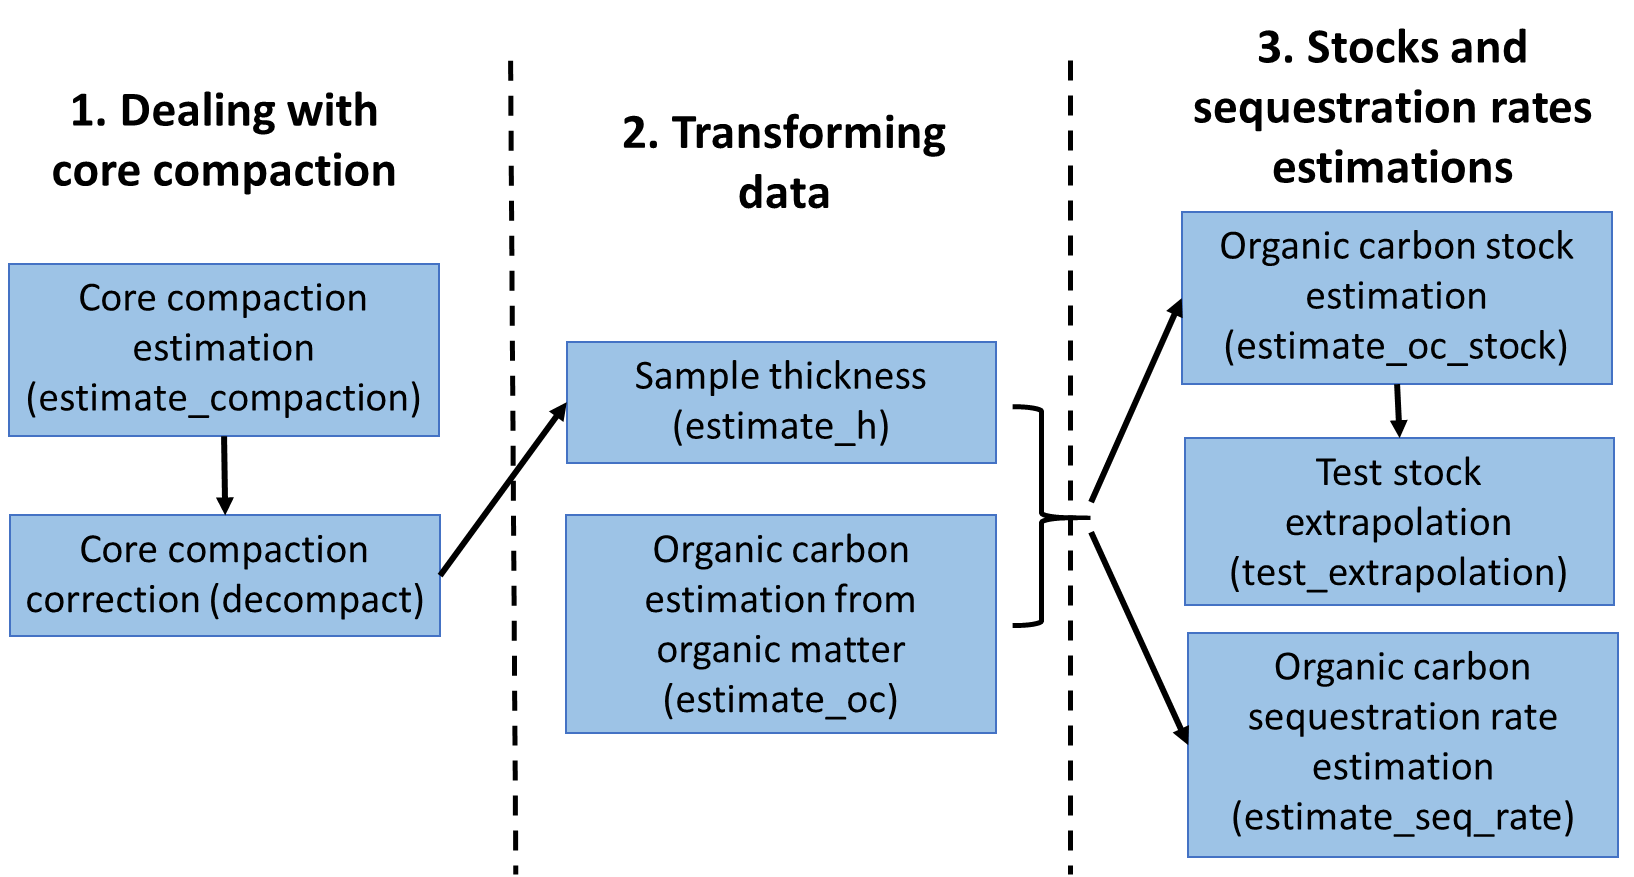
\includegraphics[keepaspectratio]{images/BC_workflow-02.png}}
\caption{Blue Carbon package workflow}
\end{figure}

\paragraph{\texorpdfstring{\textbf{\emph{estimate\_compaction}}
\textbf{- Estimate Core
Compaction}}{estimate\_compaction - Estimate Core Compaction}}\label{estimate_compaction---estimate-core-compaction}

Sampling soil cores by manual percussion often results in the compaction
of the material retrieved. This function estimates the percentage of
compaction using measurements taken before and after inserting the corer
tube (Fig. 2).

\begin{figure}
\centering
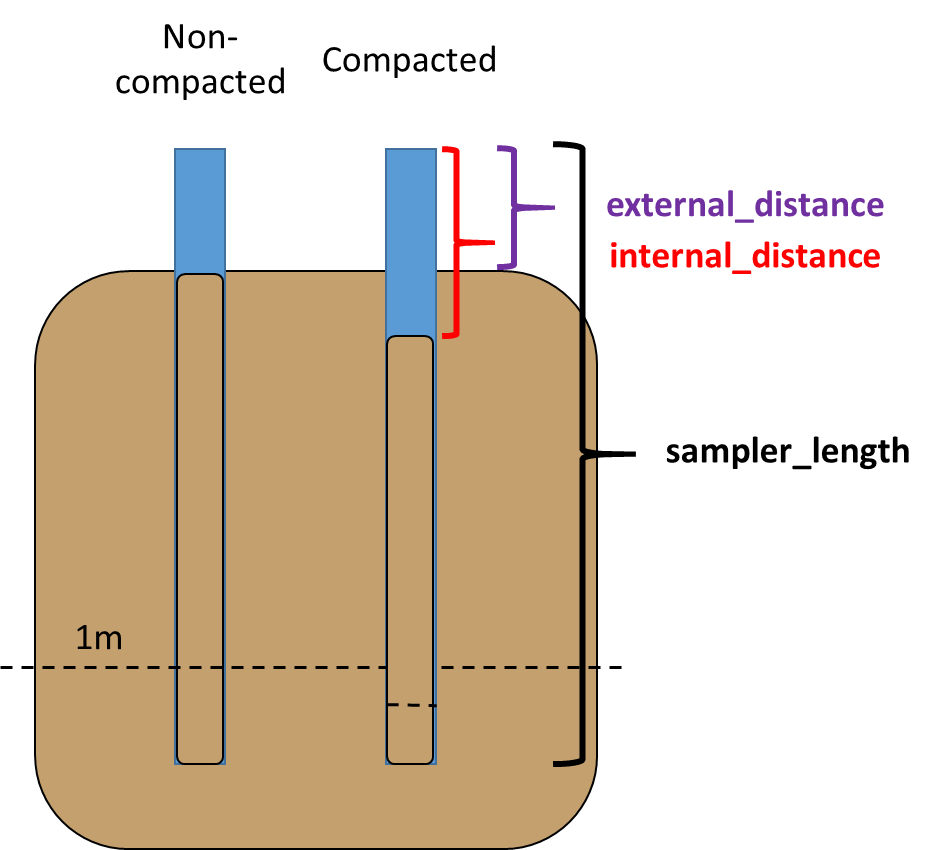
\includegraphics[width=3.51042in,height=\textheight,keepaspectratio]{images/compaction-02.png}
\caption{Soil compaction from field sampling}
\end{figure}

\paragraph{\texorpdfstring{\textbf{\emph{decompact}} \textbf{- Calculate
sediment properties after
decompaction}}{decompact - Calculate sediment properties after decompaction}}\label{decompact---calculate-sediment-properties-after-decompaction}

This function applies a linear correction (assuming uniform compaction
of the core material) to adjust the sample depth accurately. If dry bulk
density data is provided, the function also corrects it accordingly.

\paragraph{\texorpdfstring{\textbf{\emph{estimate\_oc}} \textbf{-
Organic carbon content estimation from organic carbon
data}}{estimate\_oc - Organic carbon content estimation from organic carbon data}}\label{estimate_oc---organic-carbon-content-estimation-from-organic-carbon-data}

There is a linear correlation between organic carbon and organic matter
content. This correlation can vary across ecosystems and sampling sites.
This function fits a linear regression model between organic matter and
organic carbon content of the samples and predicts organic carbon values
for samples where the latter information is missing. Estimation of
organic carbon is performed using a linear regression between the
logarithm of the organic carbon content and the logarithm of the organic
matter content (log(organic carbon) \textbackslash\textasciitilde{}
log(organic matter)), providing an organic carbon value for each organic
matter value. It fits a model for each sampling station, dominant
species, and ecosystem. If an organic carbon value is already available
for a sample, the function returns it. Otherwise, it applies the model
for the corresponding sampling station. If a model cannot be fitted for
that station (e.g.~because of limited sample size) or if the model fit
is poor, the function instead applies the model for the dominant
species. If no suitable species-level model exists, it then applies the
ecosystem-level model. If no models are available at any of these
levels, the function defaults to published models: Fourqurean et al.
(2012) for seagrasses, Maxwell et al. (2023) for salt marshes, and
Piñeiro-Juncal et al. (under review) for mangroves. It is unlikely, but
possible, that the model predicts higher organic carbon than organic
matter content. If this occurs, the function issues a warning, and it is
recommended to discard that model.

\paragraph{\texorpdfstring{\textbf{\emph{estimate\_h}} \textbf{- Sample
thickness
estimation}}{estimate\_h - Sample thickness estimation}}\label{estimate_h---sample-thickness-estimation}

For cores where only selected samples were measured, it is necessary to
assign a carbon density to the unmeasured sections before estimating the
total stock. This function identifies gaps between samples and, if any
are present, divides the space between the previous and next sample,
ensuring continuous samples without gaps in the core (Fig. 3). The
midpoint between two consecutive samples is estimated from the bottom of
the previous sample to the top of the next sample, preventing the uneven
distribution of gaps between samples with different thickness. The stock
and sequestration rate estimation functions (estimate\_oc\_stock and
estimate\_seq\_rate) already incorporate this function, so there is no
need to run it separately.

\begin{figure}
\centering
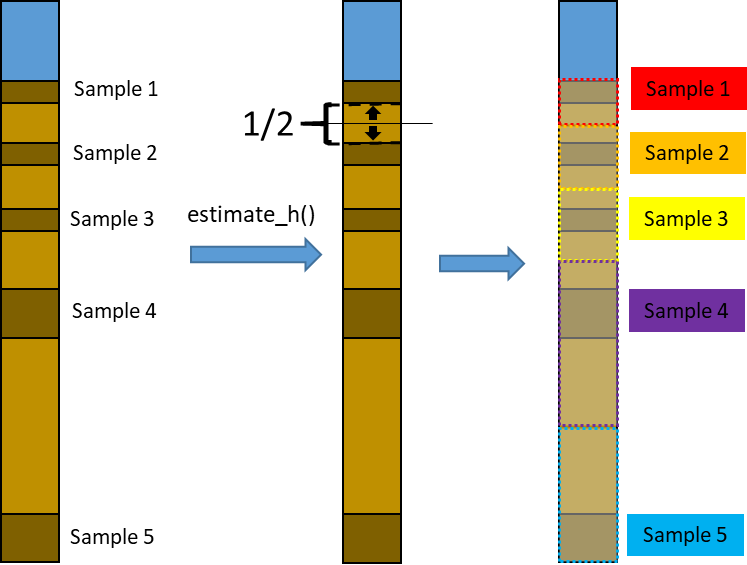
\includegraphics[width=2.79167in,height=\textheight,keepaspectratio]{images/estimate_h-01.png}
\caption{Gap distribution between samples to estimate accumulated
organic carbon mass.}
\end{figure}

\paragraph{\texorpdfstring{\textbf{\emph{estimate\_oc\_stock}} \textbf{-
Organic carbon stock
estimation}}{estimate\_oc\_stock - Organic carbon stock estimation}}\label{estimate_oc_stock---organic-carbon-stock-estimation}

Estimates carbon stocks from soil core data down to a specified depth,
with 100 as the default. If the core does not reach the desired depth,
the function extrapolates the stock using a linear model based on the
relationship between accumulated organic carbon mass and depth. In this
model, accumulated organic carbon mass (stock) is the target variable
and depth the explanatory variable (lm(accumulated organic carbon mass
\textasciitilde{} depth)).

\begin{figure}
\centering
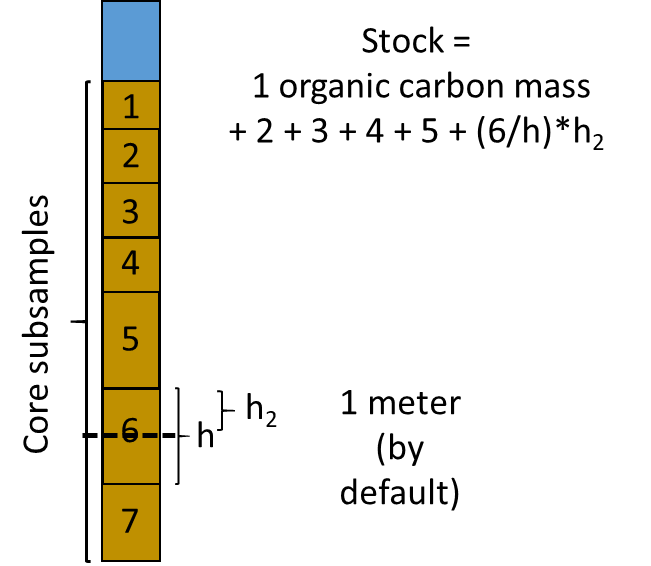
\includegraphics[width=3.25in,height=\textheight,keepaspectratio]{images/estimate_stock-01.png}
\caption{OC stock estimation diagram}
\end{figure}

\paragraph{\texorpdfstring{\textbf{\emph{test\_extrapolation}} \textbf{-
Visualize the error of stock
extrapolation}}{test\_extrapolation - Visualize the error of stock extrapolation}}\label{test_extrapolation---visualize-the-error-of-stock-extrapolation}

This function subset the cores that reach the desired depth, estimates
the observed stock, and estimates the stock using the linear model on
the relationship between accumulated organic carbon mass and depth.
Extrapolations are performed using the top 90, 75, 50 and 25\% length of
the specified depth. The function then compares the observed stock with
the extrapolated stock estimates. Note that this function requires that
at least some cores reach the desired depth.

\paragraph{\texorpdfstring{\textbf{\emph{estimate\_seq\_rate}} \textbf{-
Organic carbon sequestration rates
estimation}}{estimate\_seq\_rate - Organic carbon sequestration rates estimation}}\label{estimate_seq_rate---organic-carbon-sequestration-rates-estimation}

Estimates the average organic carbon sequestration rate in the soil over
a specified time frame (by default 100). The average sequestration rate
is calculated by dividing the stock at the depth corresponding to the
target time frame by the length of the time frame itself.

\section{Availability}\label{availability}

BlueCarbon is available in
\href{https://cran.r-project.org/package=BlueCarbon}{CRAN}. The package
documentation and expanded tutorials can be accessed
\href{https://ecologyr.github.io/BlueCarbon/}{here}. A recorded video of
a workshop and step-by-step tutorial walkthrough is available
\href{https://www.youtube.com/watch?v=XCrrR3_MSHc&ab_channel=EcoinformaticaAEET}{here}.

\section{Acknowledgements}\label{acknowledgements}

The development of this software has been funded by Fondo Europeo de
Desarrollo Regional (FEDER) and Consejería de Transformación Económica,
Industria, Conocimiento y Universidades of Junta de Andalucía (project
US-1381388 led by Francisco Rodríguez Sánchez, Universidad de Sevilla).
NPJ was supported by a Juan de la Cierva fellowship (JDC2022-048342-I,
MCIN/AEI/10.13039/501100011033, European Union
``NextGenerationEU''/PRTR''). JA acknowledges funding from the
CLIMB-FOREST Horizon Europe Project (No 101059888) funded by the
European Union. FRS was supported by VI PPIT-US from Universidad de
Sevilla. MM was supported by a FCT PhD grant
(\url{https://doi.org/10.54499/2020.06996.BD}).

\section*{References}\label{references}
\addcontentsline{toc}{section}{References}

\phantomsection\label{refs}
\begin{CSLReferences}{1}{0}
\bibitem[\citeproctext]{ref-Fourqurean_2012}
Fourqurean, J. W., Duarte, C. M., Kennedy, H., Marbà, N., Holmer, M.,
Mateo, M. A., Apostolaki, E. T., et al. (2012). Seagrass ecosystems as a
globally significant carbon stock. \emph{Nature Geoscience},
\emph{5}(7), 505--509.
doi:\href{https://doi.org/10.1038/ngeo1477}{10.1038/ngeo1477}

\bibitem[\citeproctext]{ref-Howard_2014}
Howard, J., Hoyt, S., Isensee, K., Pidgeon, E., \& Telszewski, M.
(2014). Coastal blue carbon: Methods for assessing carbon stocks and
emissions factors in mangroves, tidal salt marshes, and seagrass
meadows. \emph{Conservation International, Intergovernmental
Oceanographic Commission of UNESCO, International Union for Conservation
of Nature}.

\bibitem[\citeproctext]{ref-Maxwell_2023}
Maxwell, T. L., Rovai, A. S., Adame, M. F., Adams, J. B., Álvarez-Rogel,
J., Austin, W. E. N., Beasy, K., et al. (2023). Global dataset of soil
organic carbon in tidal marshes. \emph{Scientific Data}, \emph{10}(1),
1--14.
doi:\href{https://doi.org/10.1038/s41597-023-02633-x}{10.1038/s41597-023-02633-x}

\bibitem[\citeproctext]{ref-Piuxf1eiro-Juncal}
Piñeiro-Juncal, N., Mateo, M. Á., Leiva-Dueñas, C., Serrano, E.,
Inostroza, K., Soler, M., Apostolaki, E. T., et al. (under review). Soil
organic carbon preservation and decay trends in tidal marsh, mangrove
and seagrass blue carbon ecosystems.

\bibitem[\citeproctext]{ref-quevedo_2023}
Quevedo, J. M. D., Uchiyama, Y., \& Kohsaka, R. (2023). Progress of blue
carbon research: 12 years of global trends based on content analysis of
peer-reviewed and {``gray literature''} documents. \emph{Ocean and
Coastal Management}, \emph{236}(January), 106495.
doi:\href{https://doi.org/10.1016/j.ocecoaman.2023.106495}{10.1016/j.ocecoaman.2023.106495}

\end{CSLReferences}

\end{document}
